\documentclass{standalone}
\usepackage{tikz}
\begin{document}
    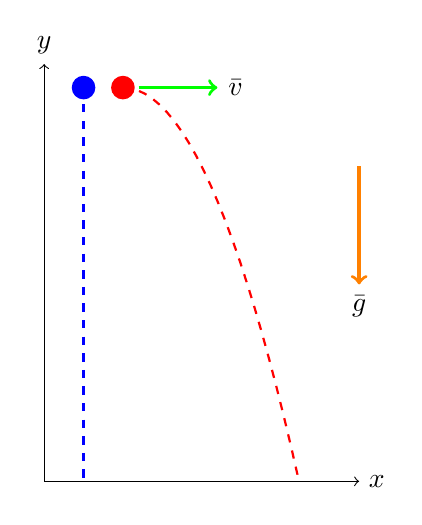
\begin{tikzpicture}
        \draw [<->] (0,5.3) node [above] {$y$} -- (0,0) -- (4,0) node [right] {$x$};
        \path [fill=blue] (0.5,5) circle [radius=0.15];
        \path [fill=red] (1,5) circle [radius=0.15];
        \draw [thick, blue, dashed] (0.5,5) -- (0.5,0);
        \draw [thick, red, dashed, domain=1:3.23] plot(\x, {-\x*\x+2*\x+4});
        \draw [very thick, green, ->] (1.2,5) -- (2.2,5) node [black, right] {$\bar{v}$};
        \draw [very thick, orange, ->] (4,4) -- (4,2.5) node [black, below] {$\bar{g}$};
    \end{tikzpicture}
\end{document}
